\documentclass[12pt]{article}

\usepackage{comment}
 
\usepackage[noend]{algpseudocode}
\usepackage{algorithm}
\usepackage{float}
\usepackage{graphicx}
\usepackage[margin=.75in]{geometry} 
\usepackage{amsmath,amsthm,amssymb}
\usepackage{amsthm}
\usepackage{mathtools,amssymb}
\usepackage{filecontents}
\usepackage{hyperref}
\usepackage{tikz}
\usepackage{tikz-3dplot}
\usetikzlibrary{shapes}
\usepackage{graphicx}
\usepackage{mathdots}
\usepackage{mathrsfs}

\newtheorem{theorem}{Theorem}
\newtheorem{definition}[theorem]{Definition}
\newtheorem{question}[theorem]{Question}
\newtheorem{example}[theorem]{Example}
\newtheorem{proposition}[theorem]{Proposition}
\newtheorem{claim}[theorem]{Claim}
\newtheorem{lemma}[theorem]{Lemma}
\newtheorem{corollary}[theorem]{Corollary}
\newtheorem{conjecture}[theorem]{Conjecture}

\newcommand{\N}{\mathbb{N}}
\newcommand{\Z}{\mathbb{Z}}
\newcommand{\R}{\mathbb{R}}
\newcommand{\C}{\mathcal{C}}
\newcommand{\D}{\mathcal{D}}
\newcommand{\PP}{\mathcal{P}}
\newcommand{\PowerSet}[1]{\mathbf{2}^{#1}}

\newcommand{\sizeof}[1]{\left\lvert{#1}\right\rvert}

\DeclareMathOperator*{\argmin}{arg\,min}
\DeclareMathOperator*{\argmax}{arg\,max}
\DeclareMathOperator{\rev}{rev}
\DeclareMathOperator{\inv}{inv}
\DeclareMathOperator{\med}{med}
\DeclareMathOperator{\topChoice}{top}
\DeclareMathOperator{\last}{last}
\DeclareMathOperator{\tg}{tg}
\DeclareMathOperator{\Cyl}{Cyl}

\newcommand{\1}[1]{\mathds{1}[{#1}]}
\renewcommand{\P}[1]{\mathds{P}\left[{#1}\right]}
\newcommand{\E}[1]{\mathds{E}\left[{#1}\right]}
\newcommand{\Var}[1]{\mathrm{Var}[{#1}]}

% This strange block is just for really nice Ps and Es functions.
\makeatletter
\newcommand\Ps@textstyle[2]{\mathbb{P}_{#1}\left[{#2}\right]}
\newcommand\Es@textstyle[2]{\mathbb{E}_{#1}\left[{#2}\right]}

\newcommand\Ps[2]{%
  \mathchoice % special stiling in display mode, regular elsewhere.
  {\underset{{#1}}{\mathbb{P}}\left[{#2}\right]
  }{\Ps@textstyle{#1}{#2}}{\Ps@textstyle{#1}{#2}}{\Ps@textstyle{#1}{#2}}
}
\newcommand\Es[2]{%
  \mathchoice % special stiling in display mode, regular elsewhere.
  {\underset{{#1}}{\mathbb{E}}\left[{#2}\right]
  }{\Es@textstyle{#1}{#2}}{\Es@textstyle{#1}{#2}}{\Es@textstyle{#1}{#2}}
}
\makeatother
\newcommand{\ip}[2]{\left\langle{#1} , {#2}\right\rangle}

\newcommand{\unit}{\mathds{1}}
\newcommand{\lo}{\succ}

\begin{document}

\title{
  Grid-Like Posets
}
\author{
  Clay Thomas \\
  claytont@cs.princeton.edu
\and
  Corey Sinnamon \\
  sinnamon@cs.princeton.edu
}

\maketitle

\section{Definitions and Basic Properties}

Define tangled grid.

\begin{definition}
  Let $\tg(n)$ denote the maximum number of downward closed sets that a tangled
  $n\times n$ grid can have.

  Let $\tg = \inf \{ \theta | \tg(n) = O( \theta^n ) \}$, i.e. $\tg$ denotes the
  base of the exponential growth of $\tg(n)$.
\end{definition}

Cite a source to prove $\tg$ is finite.

\section{A Lower Bound}

We define $\Cyl_n$, the \emph{cylinder poset} of order $n$ as follows:
its elements are pairs $\{(i,j) | i,j\in[n] \}$, and
its covering relations take two forms: 
\begin{itemize}
  \item $(i, j) \succ (i, j-1)$ for $i\in[n]$, $j\in[2,n]$. These relations
    define the ``vertical chains'' $V_i = \{ (i,j) \}_{j\in[n]}$.
  \item $(i, j) \succ (i-1, j-1)$ for $i\in[n]$, $j\in[2,n]$ and
    $(1,j) \succ (n,j-1)$ for $j\in[2,n]$. These relations form define the 
    ``diagonal chains'' $D_k = \{ (i, k + (i-1) \mod n) \}_{i\in[n]}$, where
    $\mod$ ``wraps around'' to $1$ instead of to $0$.
\end{itemize}
It's called a cylinder poset because the diagonal grids ``jump'' from one side
to the other as if the poset were on the surface of a cylinder.

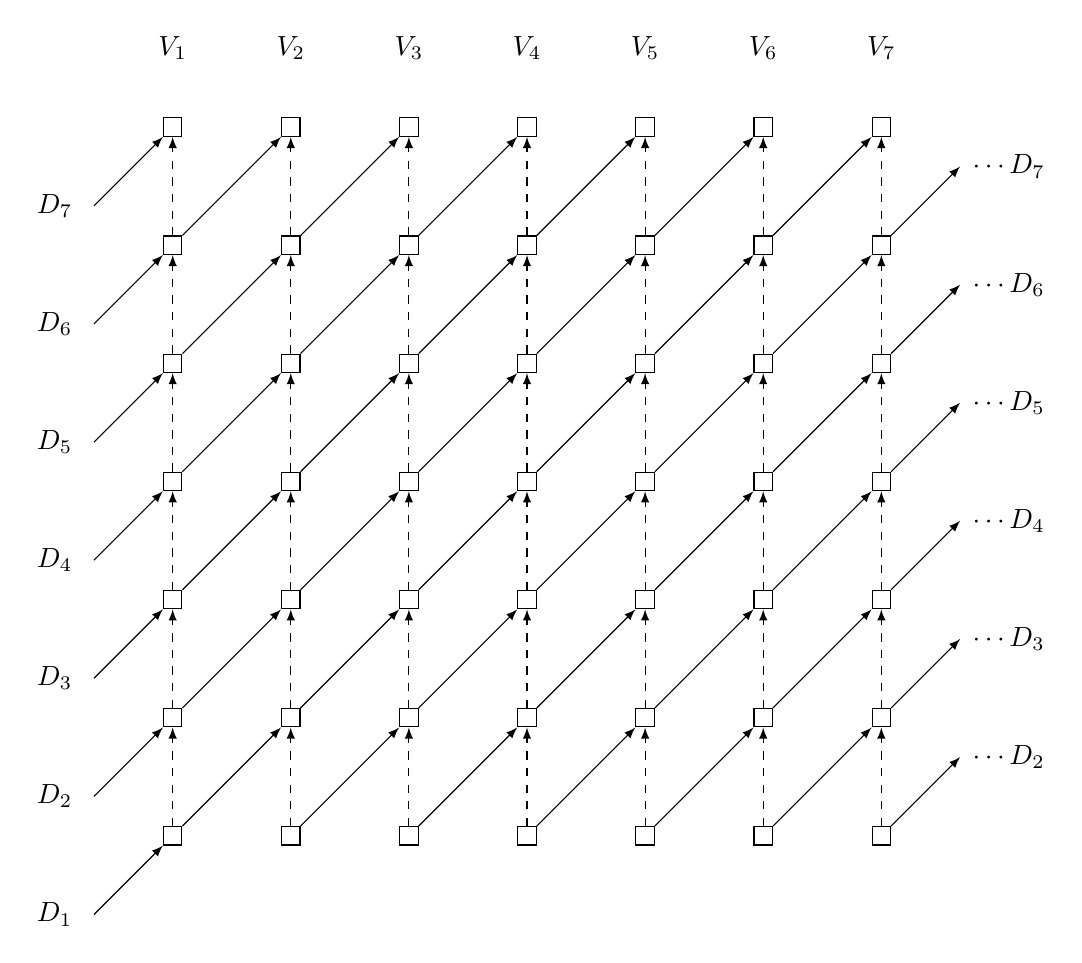
\begin{tikzpicture}
  \pgfmathtruncatemacro{\n}{7}
  \pgfmathtruncatemacro{\nD}{\n-1}
  \tikzset{>=latex}
  \foreach \x in {1,...,\n} {
    \foreach \y in {1,...,\n} {
      \node [draw]  (\x\y) at (1.5*\x,1.5*\y) {};
    }
  }
  \foreach \x in {1,...,\n} {
    \node []  (VertChain\x) at (1.5*\x,1.5*\n+1) {$V_\x$};
  }
  \foreach \y in {1,...,\n} {
    \node []  (DiagChain\y) at (0,1.5*\y-1) {$D_\y$};
    \draw [->] (0.5, 1.5*\y-1) to (1\y) ;
  }
  \foreach \y in {1,...,\nD} {
    \pgfmathtruncatemacro{\yi}{\y + 1}
    \node []  (DiagChainPrime\y) at (\n*1.5 + 1.5, 1.5*\y+1) {$\ \ \cdots D_\yi$};
    \draw [->] (\n\y) to (\n*1.5 + 1, 1.5*\y+1) ;
  }


  \foreach \x in {1,...,\nD} {
    \foreach \y in {1,...,\nD} {
      \pgfmathtruncatemacro{\yi}{\y + 1}
      \pgfmathtruncatemacro{\xi}{\x + 1}
      \draw [->, dashed] (\x\y) -- (\x\yi);
      \draw [->] (\x\y) -- (\xi\yi);
    }
  }
  \foreach \y in {1,...,\nD} {
    \pgfmathtruncatemacro{\yi}{\y + 1}
    \draw [->, dashed] (\n\y) -- (\n\yi);
  }
\end{tikzpicture}

The main result of this section is to count the number of downward closed sets
in $\Cyl_n$ using known path-counting results.

First, it's helpful to observe that there's a bijection between the downward
closed sets of $\Cyl_n$ and the set of sequences $(a_1,\ldots,a_n)$ such that
$a_i \in [0,n]$ for $i\in[n]$, $a_{i+1}\le a_i + 1$ for $i\in[n-1]$, and
$a_1\le a_n+1$. Given a downward closed set $S\subseteq \Cyl_n$, 
the bijection is given by letting $a_i$ be the height along $V_i$ of the 
highest element in $S\cap V_i$ (or zero if $S$ does not intersect $V_i$).

Now, fix $\ell$ as the height along $V_i$ of the highest element of $S\cap V_i$
(or $\ell=0$ if $S\cap V_i=\emptyset$).
Note that taking $\ell=0,1,\ldots,n$ partitions the collection of downward
closed sets. Now we identify the downward closed set $S$ with its upward
boundary in the Hasse diagram of $\Cyl_n$.
This upward boundary can then be uniquely identified with a lattice path
starting at $(1,\ell)$ where
at each node you can take an upward edge along a diagonal chain $D_k$ or a
downward edge along a vertical chain $V_i$.
This ensures that $S$ is downward closed along each $V_i$ and for the
``internal'' diagonal relations, i.e. those of the form $(i+1,j+1)\succ (i,j)$.
To satisfy the relations $(1,j+1)\succ (n,j)$, we just need the path to
terminate at $(n,\ell-1)$. To properly represent the fact that 
$S\cap V_i = \emptyset$ for a given $i$, we draw elements of height $0$ and
$-1$, and when $S\cap V_i = \emptyset$ we let the path pass through $(i-1, -1)$
and $(i,0)$. It's easy to see that a path of this form uniquely determines a
downward-closed set ((IS IT??)).

\hspace{-0.4in}
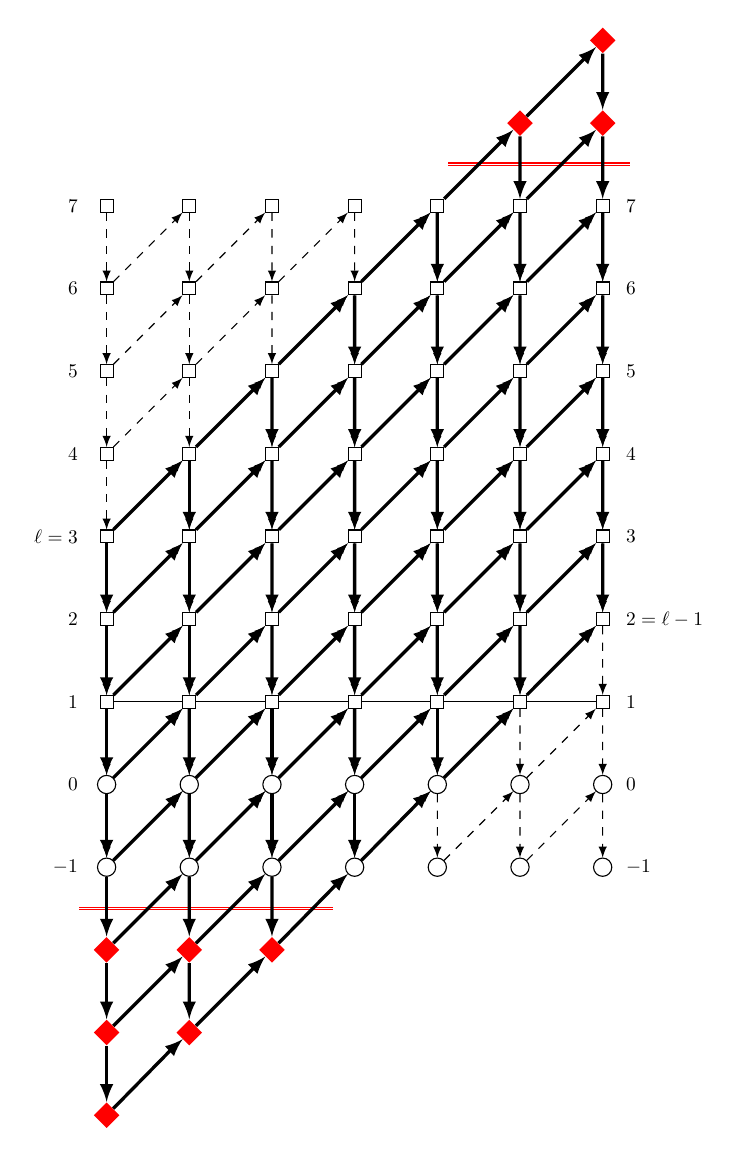
\begin{tikzpicture}[scale=0.7, every node/.style={scale=0.7}]
  \pgfmathtruncatemacro{\n}{7}
  \pgfmathtruncatemacro{\nD}{\n-1}
  \pgfmathtruncatemacro{\nU}{\n+1}
  %
  \pgfmathtruncatemacro{\l}{3}
  \pgfmathtruncatemacro{\r}{\l-1}
  %
  \tikzset{>=latex}
  \foreach \x in {1,...,\n} {
    \foreach \y in {1,...,\n} {
      \node [draw]  (\x\y) at (1.5*\x,1.5*\y) {};
    }
  }
  \foreach \x in {1,...,\n} {
    % \draw [->, dashed] (\n\y) -- (\n\yi);
    \node [draw, circle]  (\x0) at (1.5*\x, 0) {};
    \node [draw, circle]  (\x-1) at (1.5*\x, -1.5) {};
  }
  %
  \foreach \x in {2,...,\nD} {
    \foreach \y in {-1,...,\nD} {
      \pgfmathtruncatemacro{\yi}{\y + 1}
      \pgfmathtruncatemacro{\xi}{\x + 1}
      \draw [->, dashed] (\x\yi) -- (\x\y) ;
      \draw [->, dashed] (\x\y) -- (\xi\yi);
    }
  }
  \foreach \y in {-1,...,\n} {
    \ifthenelse{\y=\l}{
      \node [anchor=east] () at (1.1, 1.5*\y) {$\ell =\y$} ;
    }{ 
      \node [anchor=east] () at (1.1, 1.5*\y) {$\y$} ;
    };
    \ifthenelse{\y=\r}{
      \node [anchor=west] () at (1.5*\n + 0.3, 1.5*\y) {$\y=\ell-1$} ;
    }{ 
      \node [anchor=west] () at (1.5*\n + 0.3, 1.5*\y) {$\y$} ;
    };
  }
  \foreach \y in {-1,...,\nD} {
    \pgfmathtruncatemacro{\yi}{\y + 1}
    \draw [->, dashed] (1\y) -- (2\yi)  ;
    \draw [->, dashed] (1\yi) -- (1\y) ;
    \draw [->, dashed] (\n\yi) -- (\n\y) ;
  }
  \foreach \x in {1,...,\nD} {
    \pgfmathtruncatemacro{\xi}{\x + 1}
    \draw [] (\x1) -- (\xi1);
  }
  %
  \pgfmathtruncatemacro{\tbad}{\n-\l-1}
  \draw [double,red] (1,-1*1.5 - 0.75) to (\tbad*1.5 + 1.1, -1*1.5 - 0.75) ;
  \foreach \x in {1,...,\tbad} {
    \pgfmathtruncatemacro{\tbadheight}{ -\tbad + \x - 2 }
    \foreach \y in {\tbadheight,...,-2}{
      \node [diamond, red, fill]  (\x\y) at (1.5*\x, 1.5*\y) {};
    }
    \pgfmathtruncatemacro{\xi}{\x + 1}
  }
  %
  \pgfmathtruncatemacro{\sbad}{\l-1}
  \pgfmathtruncatemacro{\sbadstart}{\n-\sbad+1}
  \draw [double,red] (1.5*\sbadstart-1.3,\n*1.5+0.75) to (\n*1.5+0.5,\n*1.5+0.75);
  \foreach \x in {\sbadstart,...,\n} {
    \pgfmathtruncatemacro{\sbadheight}{ \x + \sbad }
    \foreach \y in {\nU,...,\sbadheight}{
      \node [diamond, red, fill]  (\x\y) at (1.5*\x, 1.5*\y) {};
    }
    \pgfmathtruncatemacro{\xi}{\x + 1}
  }
  %
  \foreach \x in {1,...,\n} {
    \pgfmathtruncatemacro{\xi}{\x + 1}
    \pgfmathtruncatemacro{\bottomHeight}{ -\tbad + \x - 2 }
    \pgfmathtruncatemacro{\topHeight}{ \l + \x - 1 }
    \foreach \y in {\bottomHeight,...,\topHeight}{
      \pgfmathtruncatemacro{\yi}{\y + 1}
      \ifthenelse{\y=\topHeight}{}{ \draw [->,very thick] (\x\yi) to (\x\y) ;};
      \ifthenelse{\x=\n}{}{ \draw [->,very thick]  (\x\y) to (\xi\yi); };
    }
    \pgfmathtruncatemacro{\xi}{\x + 1}
  }
\end{tikzpicture}
\qquad
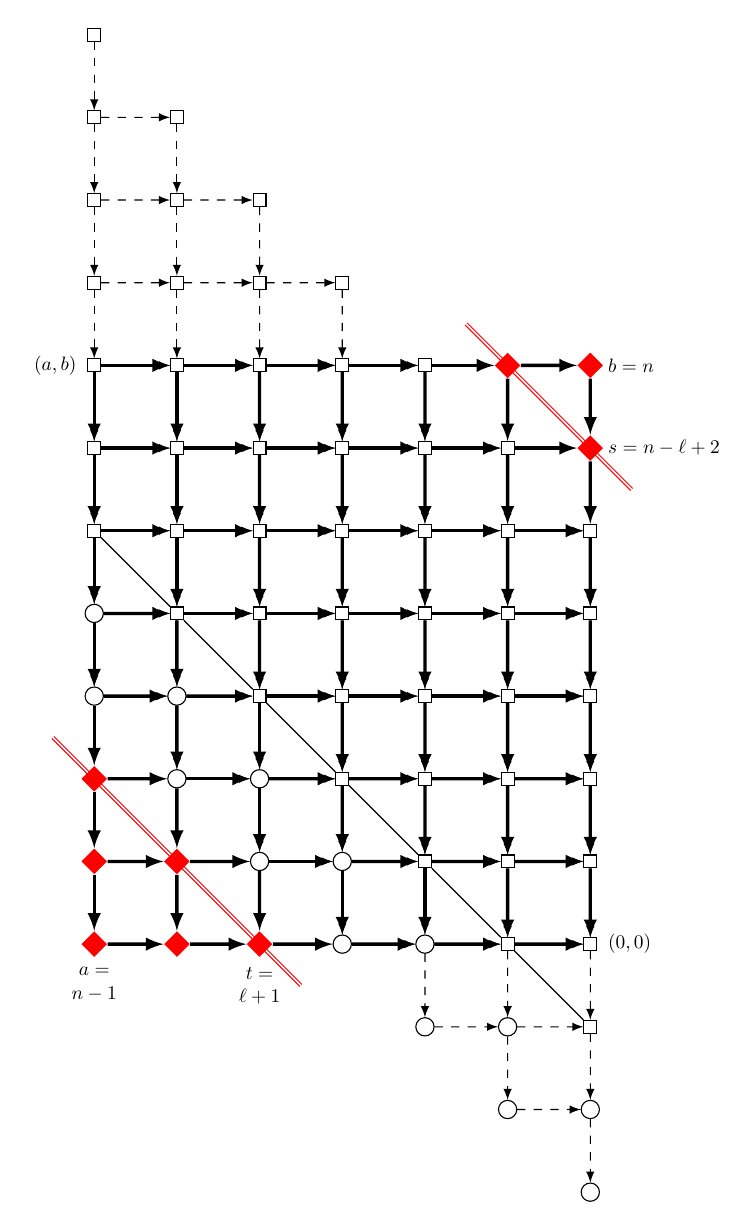
\begin{tikzpicture}[scale=0.7, every node/.style={scale=0.7}]
  \pgfmathtruncatemacro{\n}{7}
  \pgfmathtruncatemacro{\nD}{\n-1}
  \pgfmathtruncatemacro{\nU}{\n+1}
  %
  \pgfmathtruncatemacro{\l}{3}
  \pgfmathtruncatemacro{\r}{\l-1}
  %
  \tikzset{>=latex}
  \foreach \x in {1,...,\n} {
    \foreach \y in {1,...,\n} {
      \node [draw]  (\x\y) at (1.5*\x,1.5*\y-1.5*\x) {};
    }
  }
  \foreach \x in {1,...,\n} {
    % \draw [->, dashed] (\n\y) -- (\n\yi);
    \node [draw, circle]  (\x0) at (1.5*\x, -1.5*\x) {};
  }
  \foreach \x in {1,...,\n} {
    \node [draw, circle]  (\x-1) at (1.5*\x,  -1.5 + -1.5*\x ) { };
  }
  %
  %
  \foreach \x in {2,...,\nD} {
    \foreach \y in {-1,...,\nD} {
      \pgfmathtruncatemacro{\yi}{\y + 1}
      \pgfmathtruncatemacro{\xi}{\x + 1}
      \draw [->, dashed] (\x\yi) -- (\x\y) ;
      \draw [->, dashed] (\x\y) -- (\xi\yi);
    }
  }
  \foreach \y in {-1,...,\nD} {
    \pgfmathtruncatemacro{\yi}{\y + 1}
    \draw [->, dashed] (1\y) -- (2\yi)  ;
    \draw [->, dashed] (1\yi) -- (1\y) ;
    \draw [->, dashed] (\n\yi) -- (\n\y) ;
  }
  \foreach \x in {1,...,\nD} {
    \pgfmathtruncatemacro{\xi}{\x + 1}
    \draw [] (\x1) -- (\xi1);
  }
  %
  \pgfmathtruncatemacro{\tbad}{\n-\l-1}
  \draw [double,red] (0.75, -1.5*\tbad - 1.5*\l + 3*1.5 +0.75) to 
    (\tbad*1.5 + 0.75, -1.5 -0.75 +1.5*\l-1.5*\n) ;
  \foreach \x in {1,...,\tbad} {
    \pgfmathtruncatemacro{\tbadheight}{ -\tbad + \x - 2 }
    \foreach \y in {\tbadheight,...,-2}{
      \node [diamond, red, fill]  (\x\y) at (1.5*\x, 1.5*\y-1.5*\x) {};
    }
    \pgfmathtruncatemacro{\xi}{\x + 1}
  }
  %
  \pgfmathtruncatemacro{\sbad}{\l-1}
  \pgfmathtruncatemacro{\sbadstart}{\n-\sbad+1}
  \draw [double,red] (1.5*\sbadstart-0.75,\n*1.5+1.5+0.75-1.5*\sbadstart) to 
    (\n*1.5+0.75,+0.75);
  \foreach \x in {\sbadstart,...,\n} {
    \pgfmathtruncatemacro{\sbadheight}{ \x + \sbad }
    \foreach \y in {\nU,...,\sbadheight}{
      \node [diamond, red, fill]  (\x\y) at (1.5*\x, 1.5*\y-1.5*\x) {};
    }
    \pgfmathtruncatemacro{\xi}{\x + 1}
  }
  %
  \node [anchor=north, align=center] () at 
    (1.5, -1.5*\n+1.5*\sbad-0.3) {$a=$\\$n-1$} ;
  \node [anchor=north, align=center] () at 
    (1.5*\tbad, -1.5*\n+1.5*\sbad-0.3) {$t=$\\$\ell+1$} ;
  %
  \node [anchor=west, align=center] () at 
    (1.5*\n+0.2, -1.5*\n+1.5*\sbad) {$(0,0)$} ;
  \node [anchor=west, align=center] () at 
    (1.5*\n+0.2, 1.5) {$s=n-\ell+2$} ;
  \node [anchor=west, align=center] () at 
    (1.5*\n+0.2, +1.5*\sbad) {$b=n$} ;
  \node [anchor=east, align=right] () at
    (1.3, 1.5*\sbad) {$(a,b)$};
  %
  \foreach \x in {1,...,\n} {
    \pgfmathtruncatemacro{\xi}{\x + 1}
    \pgfmathtruncatemacro{\bottomHeight}{ -\tbad + \x - 2 }
    \pgfmathtruncatemacro{\topHeight}{ \l + \x - 1 }
    \foreach \y in {\bottomHeight,...,\topHeight}{
      \pgfmathtruncatemacro{\yi}{\y + 1}
      \ifthenelse{\y=\topHeight}{}{ \draw [->,very thick] (\x\yi) to (\x\y) ;};
      \ifthenelse{\x=\n}{}{ \draw [->,very thick]  (\x\y) to (\xi\yi); };
    }
    \pgfmathtruncatemacro{\xi}{\x + 1}
  }
\end{tikzpicture}

Thus, the problem is reduced to counting lattice paths in a square grid with
``missing corners'', i.e. those paths which avoid certain ``translated
diagonals'':

\begin{theorem}[Cite something]
  The number of monotonic integer lattice paths from $(0,0)$ to $(a,b)$ avoiding
  the lines $y=x+s$ and $y=x-t$ is equal to
  \[ \mathscr L(a,b;s,t) = \sum_{k\in\Z} \left[ {a+b \choose b + k(s+t)} 
      - {a+b \choose b + k(s+t) + t} \right]
    \]
  where ${u \choose v }= 0$ for $v<0$ or $v>u$.
\end{theorem}

For a fixed $n$, in the reduction to the above problem $a=n-1$ and $b=n$ are
constant. With some careful counting you see that $t=\ell+1$ and $s=n-\ell+2$
(The number of ``forbidden nodes'' in the bottom corner is $n-\ell-1$,
so $t= n-1 - (n-\ell-1) + 1$. Likewise, there are $\ell-1$ forbidden nodes in
the upper corner, so $s = n - (\ell-1) + 1$.)

Thus, the number of downward closed sets in $\Cyl_n$ is exactly
\begin{align*}
  \sum_{\ell=0}^n \mathscr L(n-1,n;n-\ell+2,\ell+1)
  & = \sum_{\ell=0}^n \sum_{k\in\Z} {2n-1 \choose n + k(n+3)} 
      - {2n-1 \choose n +\ell+1 +k(n+3)} \\
  & = \sum_{\ell=0}^n {2n-1 \choose n } 
      - {2n-1 \choose n +\ell+1 } - {2n-1 \choose \ell -2} \\
  & = (n+1){2n-1 \choose n } 
       - \sum_{\ell=0}^n {2n-1 \choose n +\ell+1 } + {2n-1 \choose \ell -2} \\
  & = (n+1){2n-1 \choose n } 
       - \left( -{2n-1 \choose n-1} - {2n-1 \choose n} +
       \sum_{k=0}^{2n-1} {2n-1 \choose k} \right) \\
  & = (n+3){2n-1 \choose n } - 2^{2n-1}
  \end{align*}

\paragraph{Acknowledgements:}
We thank Linda Cai for helpful discussions and pointing us towards valuable 
references.

\end{document}

